% Options for packages loaded elsewhere
\PassOptionsToPackage{unicode}{hyperref}
\PassOptionsToPackage{hyphens}{url}
%
\documentclass[
  ignorenonframetext,
]{beamer}
\usepackage{pgfpages}
\setbeamertemplate{caption}[numbered]
\setbeamertemplate{caption label separator}{: }
\setbeamercolor{caption name}{fg=normal text.fg}
\beamertemplatenavigationsymbolsempty
% Prevent slide breaks in the middle of a paragraph
\widowpenalties 1 10000
\raggedbottom
\setbeamertemplate{part page}{
  \centering
  \begin{beamercolorbox}[sep=16pt,center]{part title}
    \usebeamerfont{part title}\insertpart\par
  \end{beamercolorbox}
}
\setbeamertemplate{section page}{
  \centering
  \begin{beamercolorbox}[sep=12pt,center]{part title}
    \usebeamerfont{section title}\insertsection\par
  \end{beamercolorbox}
}
\setbeamertemplate{subsection page}{
  \centering
  \begin{beamercolorbox}[sep=8pt,center]{part title}
    \usebeamerfont{subsection title}\insertsubsection\par
  \end{beamercolorbox}
}
\AtBeginPart{
  \frame{\partpage}
}
\AtBeginSection{
  \ifbibliography
  \else
    \frame{\sectionpage}
  \fi
}
\AtBeginSubsection{
  \frame{\subsectionpage}
}
\usepackage{lmodern}
\usepackage{amsmath}
\usepackage{ifxetex,ifluatex}
\ifnum 0\ifxetex 1\fi\ifluatex 1\fi=0 % if pdftex
  \usepackage[T1]{fontenc}
  \usepackage[utf8]{inputenc}
  \usepackage{textcomp} % provide euro and other symbols
  \usepackage{amssymb}
\else % if luatex or xetex
  \usepackage{unicode-math}
  \defaultfontfeatures{Scale=MatchLowercase}
  \defaultfontfeatures[\rmfamily]{Ligatures=TeX,Scale=1}
\fi
\usetheme[]{CambridgeUS}
\usecolortheme{rose}
\usefonttheme{structurebold}
% Use upquote if available, for straight quotes in verbatim environments
\IfFileExists{upquote.sty}{\usepackage{upquote}}{}
\IfFileExists{microtype.sty}{% use microtype if available
  \usepackage[]{microtype}
  \UseMicrotypeSet[protrusion]{basicmath} % disable protrusion for tt fonts
}{}
\makeatletter
\@ifundefined{KOMAClassName}{% if non-KOMA class
  \IfFileExists{parskip.sty}{%
    \usepackage{parskip}
  }{% else
    \setlength{\parindent}{0pt}
    \setlength{\parskip}{6pt plus 2pt minus 1pt}}
}{% if KOMA class
  \KOMAoptions{parskip=half}}
\makeatother
\usepackage{xcolor}
\IfFileExists{xurl.sty}{\usepackage{xurl}}{} % add URL line breaks if available
\IfFileExists{bookmark.sty}{\usepackage{bookmark}}{\usepackage{hyperref}}
\hypersetup{
  pdftitle={Marc G. Genton (2001)},
  pdfauthor={Randy J},
  hidelinks,
  pdfcreator={LaTeX via pandoc}}
\urlstyle{same} % disable monospaced font for URLs
\newif\ifbibliography
\setlength{\emergencystretch}{3em} % prevent overfull lines
\providecommand{\tightlist}{%
  \setlength{\itemsep}{0pt}\setlength{\parskip}{0pt}}
\setcounter{secnumdepth}{-\maxdimen} % remove section numbering
\AtBeginSubsection{}
\AtBeginSection{}
\ifluatex
  \usepackage{selnolig}  % disable illegal ligatures
\fi

\title{Marc G. Genton (2001)}
\subtitle{Classes of Kernels for Machine Learning: A Statistics
Perspective}
\author{Randy J}
\date{8/15/2021}

\begin{document}
\frame{\titlepage}

\begin{frame}[allowframebreaks]
  \tableofcontents[hideallsubsections]
\end{frame}
\hypertarget{introduction}{%
\section{Introduction}\label{introduction}}

\begin{frame}{Introduction}
\protect\hypertarget{introduction-1}{}
Kernels allow to map the data into a high dimensional feature space in
order to increase the computational power of linear machine.

Example algorithms

\begin{itemize}
\tightlist
\item
  Support vector machines
\item
  Kernel principal component analysis
\item
  Kernel Gram-Schmidt
\item
  Bayes point machines
\item
  Gaussian processes
\end{itemize}
\end{frame}

\begin{frame}{Kernel K}
\protect\hypertarget{kernel-k}{}
\(\forall\ \pmb x,\ \pmb z \in \pmb X \subset \mathfrak R^d: \ K(\pmb x, \pmb z) = \langle \pmb\Phi(\pmb x),\ \pmb\Phi(\pmb z)\rangle\),
where \(\Phi\) is a nonlinear (or sometimes linear) map from the input
space \(\pmb X\) to the feature space \(\mathfrak F\), and
\(\langle .,\ .\rangle\) is an inner product.

\begin{itemize}
\item
  Kernel must be symmetric: \(K(\pmb x,\ \pmb z) = K(\pmb z,\ \pmb x)\)
\item
  Kernel also satisfies the Cauchy-Schwartz inequality:
  \(K^2(\pmb x,\ \pmb z) \leq K(\pmb x,\ \pmb x)K(\pmb z,\ \pmb z)\).
\item
  \emph{Mercer (1909)}: a necessary and sufficient condition for a
  symmetric function \(K(\pmb x,\ \pmb z)\) to be a kernel is that it be
  positive definite. \(\forall\ x_1,\ ... ,\ x_l\) and real numbers
  \(\lambda_1,\ ... ,\ \lambda_l\), the function \(K\) must satisfy:
  \(\sum_{i=1}^l \sum_{j=1}^l \lambda_i \lambda_j K(\pmb x_i, \pmb x_j) \leq 0 \ \ \ \ (1)\)
\end{itemize}

\emph{Symmetric positive definite functions are called covariances in
statistics.}
\end{frame}

\begin{frame}{positive defintie functions Properties}
\protect\hypertarget{positive-defintie-functions-properties}{}
\begin{enumerate}
\item
  If \(K_1\), \(K_2\) are two kernels, and \(a_1\), \(a_2\) are two
  positive real numbers, then:
  \(K(\pmb x,\ \pmb z) = a_1K_1(\pmb x,\ \pmb z) + a_2K_2(\pmb x,\ \pmb z)\ \ \ \ (2)\)
  is a kernel.
\item
  The multiplication of two kernels \(K_1\) and \(K_2\) yields a kernel:
  \(K(\pmb x,\ \pmb z) = K_1(\pmb x,\ \pmb z)K_2(\pmb x,\ \pmb z)\ \ \ \  (3)\)
\item
  Properties (2) and (3) imply that any polynomial with positive
  coefficients,
  \(pol^+(x) = \{ \sum^n_{i=1} \alpha_i x^i|n \in \mathfrak N,\ \alpha_1,\ ... ,\ \alpha_n \in \mathfrak R^+ \}\),
  evaluatedat a kernel \(K_1\), yields a kernel:
  \(K(\pmb x,\ \pmb z) = pol^+(K_1(\pmb x,\ \pmb z)) \ \ \ \ (4)\)
\end{enumerate}
\end{frame}

\begin{frame}{}
\protect\hypertarget{section}{}
\begin{enumerate}
\setcounter{enumi}{3}
\item
  In particular, we have that:
  \(K(\pmb x,\ \pmb z) = \exp(K_1(\pmb x, \pmb z)) \ \ \ \ (5)\) is a
  kernel by taking the limit of the series expansion of the exponential
  function
\item
  If \(g\) is a real-valued function on \(\pmb X\), then
  \(K(\pmb x,\ \pmb z) = g(\pmb x)g(\pmb z) \ \ \ \ (6)\) is a kernel.
\item
  If \(\psi\) is an \(\mathfrak R_p\)-valued function on \(\pmb X\) and
  \(K_3\) is a kernel on \(\mathfrak R_p \times \mathfrak R_p\), then:
  \(K(\pmb x,\ \pmb z) = K_3(\psi(\pmb x), \psi(\pmb z))\ \ \ \ (7)\) is
  also a kernel
\item
  If \(\pmb A\) is a positive definite matrix of size \(d \times d\),
  then: \(K(\pmb x,\ \pmb z) = \pmb x^{\top} \pmb A \pmb z \ \ \ \ (8)\)
  is a kernel
\end{enumerate}
\end{frame}

\begin{frame}{Extra property to construct kernels}
\protect\hypertarget{extra-property-to-construct-kernels}{}
\begin{itemize}
\item
  Let \(h\) be a real-valued function on \(\pmb X\), positive, with
  minimum at \(0\) (that is, \(h\) is a variance function). Then:
  \(K(\pmb x,\ \pmb z) = \frac {h(\pmb x + \pmb z) - h(\pmb x - \pmb z)} 4 \ \ \ \ (9)\)
  is a kernel.
\item
  The justification of (9) comes from the following identity for two
  random variables \(Y_1\) and \(Y_2\):
  \(Cov[Y_1,\ Y_2] = \frac {Var[Y_1 + Y_2] - Var[Y_1 - Y_2]} 4\).
\item
  For instance, \(h(\pmb x) = \pmb x^{\top} \pmb x\). From (9), we
  obtain the kernel:
  \(K(\pmb x,\ \pmb z) = \frac {(\pmb x + \pmb z)^{\top} (\pmb x + \pmb z) - (\pmb x - \pmb z)^{\top} (\pmb x - \pmb z)} 4 = \pmb x^{\top} \pmb z\).
\end{itemize}
\end{frame}

\hypertarget{stationary-kernels}{%
\section{Stationary Kernels}\label{stationary-kernels}}

\begin{frame}{Stationary Kernels}
\begin{itemize}
\item
  A stationary kernel is one which is translation invariant:
  \(K(\pmb x,\ \pmb z) = K_s (\pmb x - \pmb z)\), which only depends on
  the lag vector.
\item
  Also referred as ansiotropic stationary kernel, to emphasize the
  dependence on both direction and length of the lag vector.
\item
  \emph{Bochner (1955)}: \(K_s (\pmb x - \pmb z)\) is positive definite
  in \(\mathfrak R^d\) iff it has the form:
  \(K_s (\pmb x - \pmb z) = \int _{\mathfrak R^d} \cos \big(\pmb \omega ^{\top} (\pmb x - \pmb z)\big) F(d\pmb \omega) \ \ \ \ (10)\),
  where \(F\) is a positive finite measure.
\item
  The quantity \(F / K_S(\pmb 0)\) is called the spectral distribution
  function. \emph{The Fourier dual in GPML book}. Note that (10) is
  simply the Fourier transform of F.
\end{itemize}
\end{frame}

\begin{frame}{isotropic (or homogeneous) stationary kernel}
\protect\hypertarget{isotropic-or-homogeneous-stationary-kernel}{}
\begin{itemize}
\item
  When a stationary kernel depends only on the norm of the lag vector
  between two examples, and not on the direction, then the kernel is
  said to be isotropic (or homogeneous), and is thus only a function of
  distance: \(K(\pmb x,\ \pmb z) = K_I(\|x - z\|)\).
\item
  The spectral representation of isotropic stationary kernels has been
  derived from \emph{Bochner's theorem (Bochner, 1955)} by Yaglom
  (1957):
\end{itemize}

\[
K_I(\|x - z\|) = \int_0^\infty \Omega_d (\omega\|x - z\|)F(d\omega) \ \ \ \ (11)
\]

\begin{itemize}
\tightlist
\item
  where
  \(\Omega_d(x) = \Big({\frac 2 x}\Big)^{(d-2)/2} \Gamma \Big({\frac d 2}\Big) J_{(d-2)/2}(x)\),
  form a basis for functions in \(\mathfrak R^d\). Here \(F\) is any
  nondecreasing bounded function, \(\Gamma(d/2)\) is the gamma function,
  and \(J_v\) is the Bessel function of the first kind of order \(v\).
\end{itemize}
\end{frame}

\begin{frame}{isotropic (or homogeneous) stationary kernel}
\protect\hypertarget{isotropic-or-homogeneous-stationary-kernel-1}{}
\begin{itemize}
\item
  Some familiar examples of \(\Omega_d\) are \(\Omega_1(x) = \cos(x)\),
  \(\Omega_2(x) = J_0(x)\), and \(\Omega_3(x) = \sin(x)/x\).
\item
  By choosing a nondecreasing bounded function \(F\) (or its derivative
  \(f\)), we can derive the corresponding kernel from (11). For instance
  in \(\mathfrak R^1\), with the spectral density
  \(f(\omega) = (1 - \cos(\omega))/(\pi \omega_2)\), we derive the
  triangular kernel:
\end{itemize}

\[
K_I(\pmb x - \pmb z) = \int_0^\infty \cos(\omega|x - z|) \frac {1 - \cos(\omega)} {\pi \omega^2} d\omega = {\frac 1 2} (1 - |x - z|)^+
\]

where \((x)^+ = max(x,\ 0)\) (see \emph{Figure 1}).
\end{frame}

\begin{frame}{}
\protect\hypertarget{section-1}{}
\begin{center}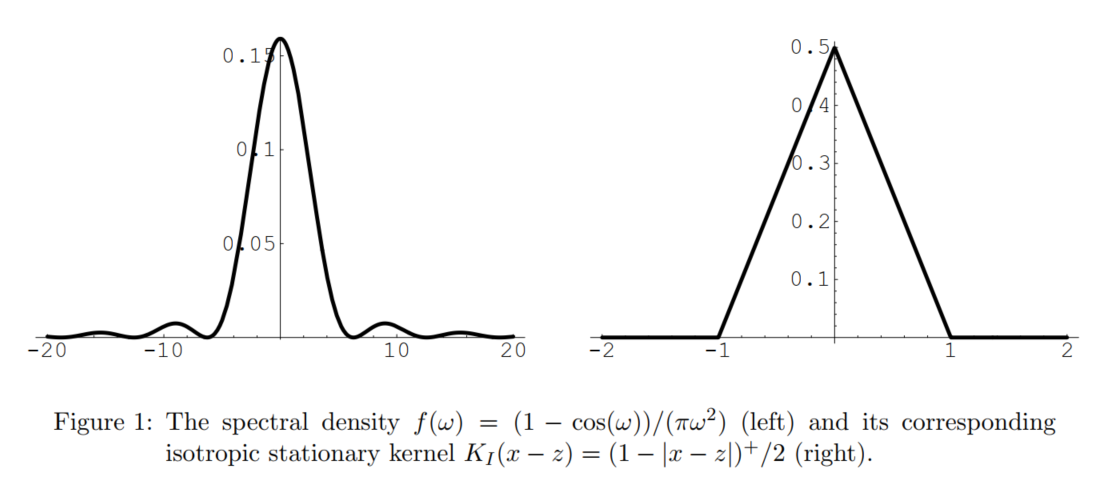
\includegraphics[width=0.8\linewidth]{figure/marc_f1} \end{center}
\end{frame}

\begin{frame}{}
\protect\hypertarget{section-2}{}
\begin{itemize}
\item
  Note that an isotropic stationary kernel obtained with \(\Omega_d\) is
  positive definite in \(\mathfrak R^d\) and in lower dimensions, but
  not necessarily in higher dimensions.
\item
  For example, the kernel \(K_I(\pmb x - \pmb z) = (1 - |x - z|)^+/2\)
  is positive definite in \(\mathfrak R^1\) but not in
  \(\mathfrak R^2\).
\item
  It is interesting to remark from (11) that an isotropic stationary
  kernel has a lower bound \emph{(Stein, 1999)}:
  \(K_I(\|\pmb x - \pmb z\|)/K_I(0) \geq \inf_{x \geq 0} \Omega_d(x)\),
  thus yielding:

  \begin{itemize}
  \tightlist
  \item
    \(K_I(\|\pmb x - \pmb z\|)/K_I(0) \geq -1\ in\ \mathfrak R^1\)\\
  \item
    \(K_I(\|\pmb x - \pmb z\|)/K_I(0) \geq -0.403\ in\ \mathfrak R^2\)\\
  \item
    \(K_I(\|\pmb x - \pmb z\|)/K_I(0) \geq -0.218\ in\ \mathfrak R^3\)\\
  \item
    \(K_I(\|\pmb x - \pmb z\|)/K_I(0) \geq 0\ in\ \mathfrak R^\infty\)
  \end{itemize}
\end{itemize}
\end{frame}

\begin{frame}{}
\protect\hypertarget{section-3}{}
\begin{itemize}
\item
  The isotropic stationary kernels must fall off more quickly as the
  dimension d increases, as might be expectedby examining the basis
  functions \(\Omega_d\). Those in \(R^\infty\) have the greatest
  restrictions placedon them.
\item
  Isotropic stationary kernels that are positive definite in
  \(\mathfrak R^d\) form a nested family of subspaces. When
  \(d \rightarrow \infty\) the basis \(\Omega_d(x)\) goes to
  \(\exp(-x^2)\).
\item
  \emph{Schoenberg (1938)}: if \(\beta_d\) is the class of positive
  definite functions of the form given by \emph{Bochner (1955)}, then
  the classes for all \(d\) have the property:
  \(\beta_1 \subset \beta_2 \subset \ ...\ \subset \beta_d \subset ...\ \subset \beta_\infty\),
  so that as \(d\) is increased, the space of available functions is
  reduced.
\end{itemize}
\end{frame}

\begin{frame}{Commonly used isotropic stationary kernels
\(K_I(\|\pmb x - \pmb z\|)/K_I(0)\)}
\protect\hypertarget{commonly-used-isotropic-stationary-kernels-k_ipmb-x---pmb-zk_i0}{}
\begin{block}{(a) Circular:}
\protect\hypertarget{a-circular}{}
positive definite in \(\mathfrak R^2\)
\({\frac 2 \pi} \arccos \Big(\frac {\|\pmb x - \pmb z\|} \theta \Big) - {\frac 2 \pi} \frac {\|\pmb x - \pmb z\|} \theta \sqrt {1 - \Big(\frac {\|\pmb x - \pmb z\|} \theta \Big)^2}\)
if \(\|\pmb x - \pmb z\| < \theta\) zero otherwise

\begin{center}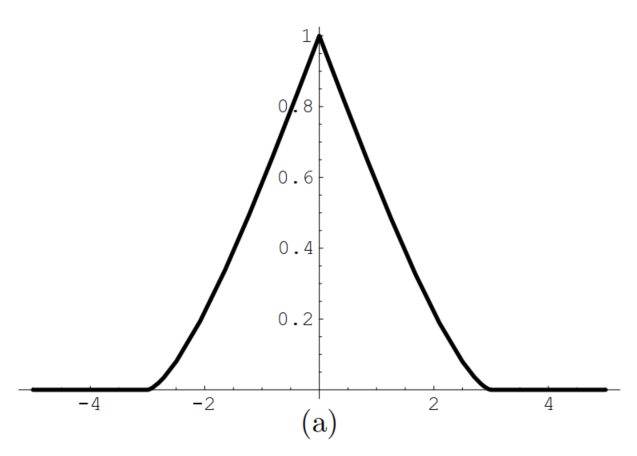
\includegraphics[width=0.5\linewidth]{figure/marc_f2a} \end{center}
\end{block}
\end{frame}

\begin{frame}{}
\protect\hypertarget{section-4}{}
\begin{block}{(b) Spherical:}
\protect\hypertarget{b-spherical}{}
positive definite in \(\mathfrak R^3\)
\(1 - {\frac 3 2} \frac {\|\pmb x - \pmb z\|} \theta + {\frac 1 2} \Big(\frac {\|\pmb x - \pmb z\|} \theta \Big)^3\)
if \(\|\pmb x - \pmb z\| < \theta\) zero otherwise

\begin{center}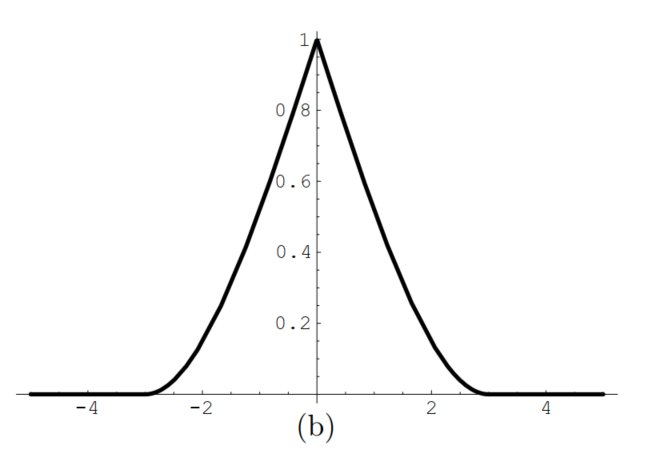
\includegraphics[width=0.5\linewidth]{figure/marc_f2b} \end{center}
\end{block}
\end{frame}

\begin{frame}{}
\protect\hypertarget{section-5}{}
\begin{block}{(c) Rational quadratic:}
\protect\hypertarget{c-rational-quadratic}{}
positive definite in \(\mathfrak R^d\)
\(1 - \frac {\|\pmb x - \pmb z\|^2} {\|\pmb x - \pmb z\|^2 + \theta}\)

\begin{center}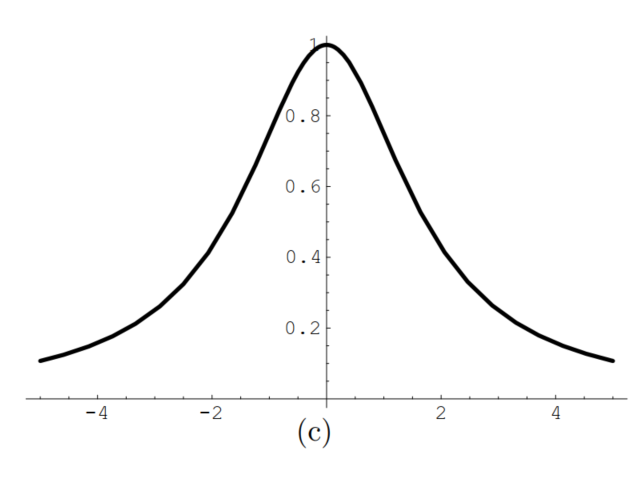
\includegraphics[width=0.5\linewidth]{figure/marc_f2c} \end{center}
\end{block}
\end{frame}

\begin{frame}{}
\protect\hypertarget{section-6}{}
\begin{block}{(d) Exponential:}
\protect\hypertarget{d-exponential}{}
positive definite in \(\mathfrak R^d\)
\(\exp \Big(- \frac {\|\pmb x - \pmb z\|} \theta \Big)\)

\begin{center}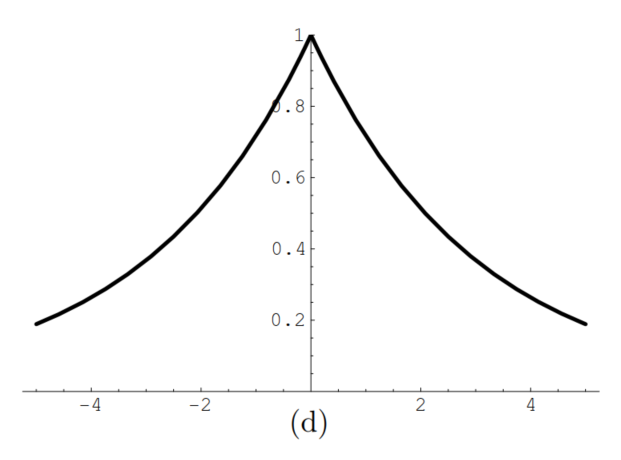
\includegraphics[width=0.5\linewidth]{figure/marc_f2d} \end{center}
\end{block}
\end{frame}

\begin{frame}{}
\protect\hypertarget{section-7}{}
\begin{block}{(e) Gaussian:}
\protect\hypertarget{e-gaussian}{}
positive definite in \(\mathfrak R^d\)
\(\exp \Big(- \frac {\|\pmb x - \pmb z\|^2} \theta \Big)\)

\begin{center}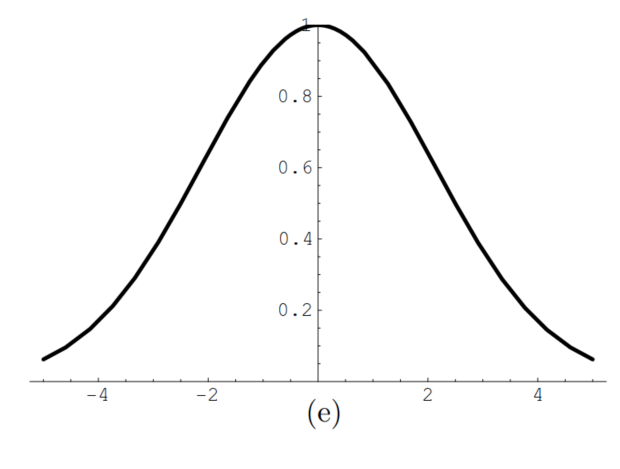
\includegraphics[width=0.5\linewidth]{figure/marc_f2e} \end{center}
\end{block}
\end{frame}

\begin{frame}{}
\protect\hypertarget{section-8}{}
\begin{block}{(f) Wave:}
\protect\hypertarget{f-wave}{}
positive definite in \(\mathfrak R^3\)
\(\frac {\theta} {\|\pmb x - \pmb z\|} \sin \Big(\frac {\|\pmb x - \pmb z\|} \theta \Big)\)

\begin{center}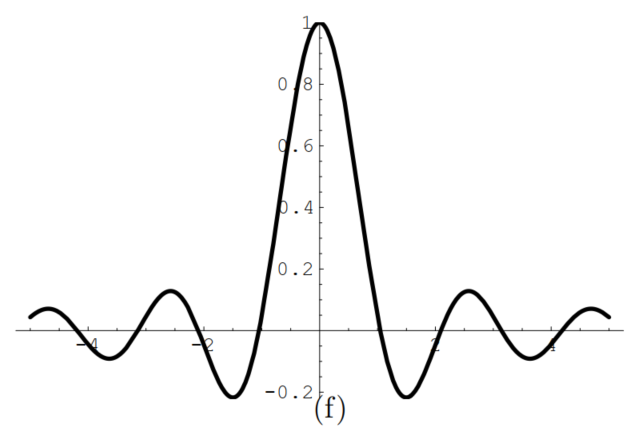
\includegraphics[width=0.5\linewidth]{figure/marc_f2f} \end{center}
\end{block}
\end{frame}

\begin{frame}{}
\protect\hypertarget{section-9}{}
\begin{itemize}
\item
  \(\theta > 0\) as a scale parameter:
\item
  The exponential kernel (d) is obtained from the spectral
  representation (11) with the spectral density:
  \(f(\omega) = \frac 1 {{\frac \pi \theta} + \pi \theta\omega^2}\)
\item
  The Gaussian kernel (e) is obtained with the spectral density:
  \(f(\omega) = \frac {\sqrt \theta} {2\sqrt \pi} \exp \Big(-\frac {\theta\omega^2} 4\Big)\).
\item
  Note also that the circular and spherical kernels have compact
  support. They have a linear behavior at the origin, which is also true
  for the exponential kernel.
\item
  The rational quadratic, Gaussian, and wave kernels have a parabolic
  behavior at the origin. This indicates a different degree of
  smoothness.
\end{itemize}
\end{frame}

\begin{frame}{Matern kernel}
\protect\hypertarget{matern-kernel}{}
\begin{itemize}
\item
  The Matern kernel \emph{(Matern, 1960)} has recently received
  considerable attention, because it allows to control the smoothness
  with a parameter \(\nu\).
\item
  The Matern kernel is defined by:
\end{itemize}

\[
K_I(\|\pmb x - \pmb z\|)/K_I(0) = {\frac 1 {2^{\nu-1}\Gamma(\nu)}} \Big(\frac {2\sqrt \nu\|\pmb x - \pmb z\|} {\theta} \Big)^\nu H_\nu \Big(\frac {2\sqrt \nu\|\pmb x - \pmb z\|} {\theta} \Big) \ \ \ \ (12)
\]

where \(\Gamma\) is the Gamma function and \(H_\nu\) is the modified
Bessel function of the second kind of order \(\nu\).

\begin{itemize}
\tightlist
\item
  Note that the Matern kernel reduces to the exponential kernel for
  \(\nu = 0.5\) and to the Gaussian kernel for
  \(\nu \rightarrow \infty\).
\end{itemize}
\end{frame}

\begin{frame}{Compactly supported kernels}
\protect\hypertarget{compactly-supported-kernels}{}
\begin{itemize}
\item
  Compactly supported kernels are kernels that vanish whenever the
  distance between two examples \(\pmb x\) and \(\pmb z\) is larger than
  a certain cut-off distance, often called the range.
\item
  For instance, the spherical kernel (b) is a compactly supported kernel
  since \(K_I(\|\pmb x - \pmb z\|) = 0\) when
  \(\|\pmb x - \pmb z\| \geq \theta\). This might prove a crucial
  advantage for certain applications dealing with massive data sets,
  because the corresponding Gram matrix \(G\),
  \(G_{ij} = K(\pmb x_i,\ \pmb x_j)\), will be sparse.
\item
  Then, linear systems involving the matrix \(G\) can be solved very
  efficiently using sparse linear algebra techniques, seen \emph{Gilbert
  et al.(1992)}.
\end{itemize}
\end{frame}

\begin{frame}{Example}
\protect\hypertarget{example}{}
\begin{center}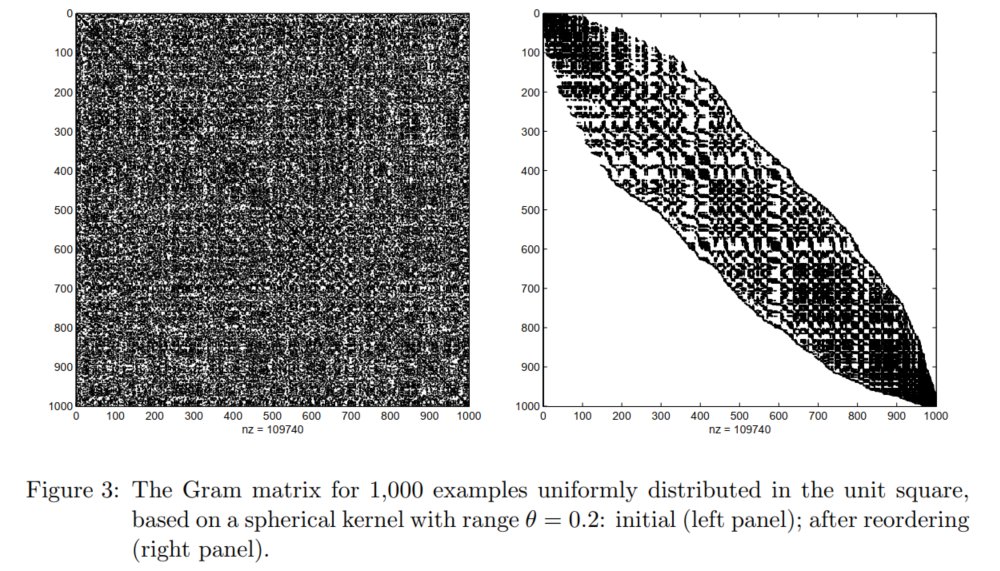
\includegraphics[width=0.8\linewidth]{figure/marc_f3} \end{center}
\end{frame}

\begin{frame}{Example (continued)}
\protect\hypertarget{example-continued}{}
\begin{itemize}
\item
  The reordered Gram matrix has now a bandwidth of only 252 instead of
  1,000 for the initial matrix, andimportant computational savings can
  be obtained.
\item
  A compactly supported kernel of Matern type can be obtained by
  multiplying the kernel (12) by the kernel:
  \(\max \Big\{ \big(1 - \frac {\|\pmb x - \pmb z\|} {\tilde \theta} \big)^{\tilde \nu},\ 0\Big\}\),
  where \(\tilde \theta > 0\) and \(\tilde \nu \geq (d + 1)/2\), in
  order to insure positive definiteness.
\item
  This product is a kernel by the property (3). Beware that it is not
  possible to simply ``cut-off'' a kernel in order to obtain a compactly
  supported one, because the result will not be positive definite in
  general.
\end{itemize}
\end{frame}

\hypertarget{locally-stationary-kernels}{%
\section{Locally Stationary Kernels}\label{locally-stationary-kernels}}

\begin{frame}{Locally Stationary Kernels}
\protect\hypertarget{locally-stationary-kernels-1}{}
\emph{(Silverman, 1957, 1959)}: \[
K(\pmb x,\ \pmb z) = K_1 \Big(\frac {\pmb x + \pmb z} 2 \Big) K_2(\pmb x - \pmb z) \ \ \ \ (13)
\]

\begin{itemize}
\item
  where \(K_1\) is a nonnegative function and \(K_2\) is a stationary
  kernel. Note that if \(K_1\) is a positive constant, then (13) reduces
  to a stationary kernel.
\item
  Further impose that \(K_2(\pmb 0) = 1\). The variable
  \((\pmb x + \pmb z)/2\) has been chosen because of its suggestive
  meaning of the average or centroidof the examples \(\pmb x\) and
  \(\pmb z\).
\end{itemize}
\end{frame}

\begin{frame}{}
\protect\hypertarget{section-10}{}
\begin{itemize}
\item
  The variance is determined by:
  \(K(\pmb x,\ \pmb x) = K_1(\pmb x)K_2(\pmb 0) = K_1(\pmb x)\ \ \  (14)\)
  thus justifying the name of power schedule for \(K_1(x)\), which
  describes the global structure.
\item
  On the other hand, \(K_2(\pmb x-\pmb z)\) is invariant under shifts
  and thus describes the local structure. It can be obtained by
  considering:
  \(K(\pmb x/2,\ -\pmb x/2) = K_1(\pmb 0)K_2(\pmb x) \ \ \ \ (15)\)
\end{itemize}
\end{frame}

\begin{frame}{Properties}
\protect\hypertarget{properties}{}
\begin{itemize}
\tightlist
\item
  Equations (14) and (15) imply that the kernel \(K(\pmb x,\ \pmb z)\)
  defined by (13) is completely determinedby its values on the diagonal
  \(\pmb x = \pmb z\) and antidiagonal \(\pmb x = - \pmb z\), for:
\end{itemize}

\[
K(\pmb x,\ \pmb z) = \frac {K \big({\frac {(\pmb {x + z})} 2},\ {\frac {(\pmb {x + z})} 2}\big)K \big({\frac {(\pmb {x - z})} 2},\ -{\frac {(\pmb {x - z})} 2}\big)} {K(\pmb 0,\ \pmb 0)} \ \ \ \ (16)
\]

\begin{itemize}
\item
  \(K_1\) is invariant with respect to shifts parallel to the
  antidiagonal, whereas \(K_2\) is invariant with respect to shifts
  parallel to the diagonal.
\item
  These properties allow to find moment estimators of both \(K_1\) and
  \(K_2\) from a single realization of data, although the kernel is not
  stationary.
\end{itemize}
\end{frame}

\begin{frame}{}
\protect\hypertarget{section-11}{}
\begin{itemize}
\item
  Another special class of locally stationary kernels is defined by
  kernels of the form: \(K(\pmb x,\ \pmb z) = K_1(x + z) \ \ \ \ (17)\)
  the so-called exponentially convex kernels \emph{(Loeve, 1946, 1948)}.
\item
  From (16), we see immediately that \(K_1(\pmb x + \pmb z) \geq 0\).
  Actually, as notedby Loeve, any two-sided Laplace transform of a
  nonnegative function is an exponentially convex kernel.
\end{itemize}
\end{frame}

\begin{frame}{}
\protect\hypertarget{section-12}{}
\begin{itemize}
\item
  A large class of locally stationary kernels can therefore be
  constructed by multiplying an exponentially convex kernel by a
  stationary kernel, since the product of two kernels is a kernel by the
  property (3).
\item
  However, the following example is a locally stationary kernel in
  \(\mathfrak R^1\) which is not the product of two kernels:
  \(\exp[-a(x^2+z^2)]=\exp \Big[-2a\big(\frac {x+z} 2\big)^2\Big] \exp\Big[-\frac {a(x+z)^2} 2\Big],\ a>0 \ \ \ \ (18)\)
  since the first factor in the right side is a positive function
  without being a kernel, and the second factor is a kernel.
\end{itemize}
\end{frame}

\begin{frame}{}
\protect\hypertarget{section-13}{}
\begin{itemize}
\item
  Finally, with the positive definite Delta kernel
  \(\delta(\pmb x - \pmb z)\), which is equal to 1 if
  \(\pmb x = \pmb z\) and 0 otherwise, the product:
  \(K(\pmb x,\ \pmb z) = K_1\Big(\frac {\pmb x + \pmb z} 2\Big) \delta(\pmb x - \pmb z)\),
  is a locally stationary kernel, often called a \emph{locally
  stationary white noise}.
\item
  The spectral representation of locally stationary kernels has
  remarkable properties. Indeed, it can be written as \emph{(Silverman,
  1957)}:
  \(K(\pmb x,\ \pmb z) = \int_{\mathfrak R^d} \int_{\mathfrak R^d} \cos(\pmb \omega^{\top}_1 \pmb x - \pmb\omega ^{\top}_2 \pmb z) f_1\big(\frac {\pmb\omega_1+\pmb\omega_2} 2\big) f_2(\pmb\omega_1-\pmb\omega_2)d\pmb\omega_1d\pmb\omega_2\),
\item
  i.e.~the spectral density
  \(f_1\big(\frac{\pmb\omega_1+\pmb\omega_2}{2}\big)f_2(\pmb\omega_1-\pmb\omega_2)\)
  is also a locally stationary kernel, and:
\end{itemize}

\[
K_1(\pmb u)=\int_{\mathfrak R^d}\cos(\pmb\omega^{\top}\pmb u)f_2(\pmb\omega)d\pmb\omega
\] \vspace{5mm} \[
K_2(\pmb v)=\int_{\mathfrak R^d}\cos(\pmb\omega^{\top}\pmb v)f_1(\pmb\omega)d\pmb\omega
\]
\end{frame}

\begin{frame}{}
\protect\hypertarget{section-14}{}
\begin{itemize}
\tightlist
\item
  i.e.~\(K_1\), \(f_2\) and \(K_2\), \(f_1\) are Fourier transform
  pairs. For instance, to the locally stationary kernel (18) corresponds
  the spectral density:
\end{itemize}

\tiny

\[
f_1\big(\frac{\omega_1 + \omega_2}{2}\big)f_2(\omega_1 - \omega_2)={\frac 1 {4\pi a}}\exp \Big[-\frac 1{2a}\big(\frac {(\omega_1 + \omega_2)} 2\big)^2\Big] \exp\Big[-\frac 1{8a} \frac {(\omega_1 - \omega_2)^2}2\Big]
\]

\normalsize

\begin{itemize}
\item
  This is immediately seen to be locally stationary since, except for a
  positive factor, it is of the form (18), with a replaced by
  \(1/(4a)\).
\item
  In particular, we can obtain a very rich family of locally stationary
  kernels by multiplying a Matern kernel (12) by an exponentially convex
  kernel (17). The resulting product is still a kernel by the property
  (3).
\end{itemize}
\end{frame}

\hypertarget{nonstationary-kernels}{%
\section{Nonstationary Kernels}\label{nonstationary-kernels}}

\begin{frame}{Nonstationary kernels}
\protect\hypertarget{nonstationary-kernels-1}{}
\begin{itemize}
\item
  The most general class of kernels is the one of nonstationary kernels,
  \(K(\pmb x,\ \pmb z)\).
\item
  For example, the polynomial kernel of degree \(p\):
  \(K(\pmb x,\ \pmb z) = (\pmb x^{\top}\pmb z)^p\), is a nonstationary
  kernel. The spectral representation of nonstationary kernels is very
  general. A nonstationary kernel \(K(\pmb x,\ \pmb z)\) is positive
  definite in \(\mathfrak R^d\) if and only if it has the form
  \emph{(Yaglom, 1987)}: where \(F\) is a positive bounded symmetric
  measure.
\end{itemize}

\[
K(\pmb x,\ \pmb z) = \int_{\mathfrak R^d} \int_{\mathfrak R^d} \cos(\pmb\omega_1^{\top} \pmb x-\pmb\omega_2^{\top} \pmb z)F (d\pmb\omega_1, d\pmb\omega_2)\ \ \ \ (19)
\]

\begin{itemize}
\tightlist
\item
  When the function \(F(\pmb \omega_1, \pmb\omega_2)\) is concentrated
  on the diagonal \(\omega_1 = \omega_2\), then (19) reduces to the
  spectral representation (10) of stationary kernels. Here again, many
  nonstationary kernels can be constructed with (19).
\end{itemize}
\end{frame}

\begin{frame}{}
\protect\hypertarget{section-15}{}
\begin{itemize}
\item
  Of interest are nonstationary kernels obtainedfrom (19) with
  \(\pmb \omega_1 = \pmb \omega_2\) but with a spectral density that is
  not integrable in a neighborhoodaroundthe origin. Such kernels are
  referred to as generalized kernels \emph{(Matheron, 1973)}.
\item
  For instance, the Brownian motion generalized kernel corresponds to a
  spectral density \(f(\omega) = 1/\|\omega\|^2\) \emph{(Mandelbrot and
  Van Ness, 1968)}.
\item
  A particular family of nonstationary kernels is the one of separable
  nonstationary kernels:
  \(K(\pmb x,\ \pmb z) = K_1(\pmb x)K_2(\pmb z)\), where \(K_1\) and
  \(K_2\) are stationary kernels evaluated at the examples \(\pmb x\)
  and \(\pmb z\) respectively.
\end{itemize}
\end{frame}

\begin{frame}{}
\protect\hypertarget{section-16}{}
\begin{itemize}
\item
  Separable nonstationary kernels possess the property that their Gram
  matrix \(G\), with \(G_{ij}=K(\pmb x_i, \pmb x_j)\), can be written as
  a tensor product (also called Kronecker product, see \emph{Graham,
  1981}) of two vectors defined by \(K_1\) and \(K_2\) respectively.
\item
  This is especially useful to reduce computational burden when dealing
  with massive data sets. For instance, consider a set of \(l\) examples
  \(\pmb x_1,\ ... ,\ \pmb x_l\). The memory requirements for the
  computation of the Gram matrix is reduced from \(l^2\) to \(2l\) since
  it suffices to evaluate the vectors
  \(\pmb a=\big(K_1(\pmb x_1),\ ...,\ K_1(\pmb x_l)\big)^{\top}\) and
  \(\pmb b=\big(K_2(\pmb x_1),\ ...,\ K_2(\pmb x_l)\big)^{\top}\).
\item
  We then have \(G = \pmb{ab}^{\top}\). Such a computational reduction
  can be of crucial importance for certain applications involving very
  large training sets.
\end{itemize}
\end{frame}

\hypertarget{reducible-kernels}{%
\section{Reducible Kernels}\label{reducible-kernels}}

\begin{frame}{Main idea}
\protect\hypertarget{main-idea}{}
\begin{itemize}
\item
  To find a new feature space where stationarity (see \emph{Sampson and
  Guttorp, 1992}) or local stationarity (see \emph{Genton and Perrin,
  2001}) can be achieved.
\item
  A nonstationary kernel \(K(\pmb x,\ \pmb z)\) is stationary reducible
  if there exist a bi-jective deformation \(\pmb \Phi\) such that:
  \(K(\pmb x,\ \pmb z) = K_S^*(\pmb\Phi(\pmb x) - \pmb\Phi(\pmb z))\ \ \ \ (20)\)
  where \(K_S^*\) is a stationary kernel.
\item
  For example in \(\mathfrak R^2\), the nonstationary kernel defined by:
  \(K(\pmb x,\ \pmb z) = \frac {\|\pmb x\| + \|\pmb z\| - \|\pmb z - \pmb x\|}{2 \sqrt{\|\pmb x\|\|\pmb z\|}} \ \ \ \ (21)\)
  is stationary reducible with the deformation:
  \(\pmb \Phi(\pmb x_1, \pmb x_2) = \bigg(\ln\Big(\sqrt {x^2_1+x^2_2}\Big),\ \arctan(x_2/x_1)\bigg)^{\top}\),
  yielding the stationary kernel:
\end{itemize}

\[
K_S^*(\pmb u_1, \pmb u_2) = \cosh(\frac{\pmb u_1} 2) - \sqrt{\frac {\cosh(\frac {\pmb u1} 2) - \cos(\pmb u_2)} 2} \ \ \ \ (22)
\]
\end{frame}

\begin{frame}{}
\protect\hypertarget{section-17}{}
\begin{itemize}
\item
  Effectively, it is straightforward to check with some algebra that
  (22) evaluated at:
  \(\pmb\Phi(\pmb x) - \pmb\Phi(\pmb z) = \bigg( \ln\Big(\frac {\|\pmb x\|}{\|\pmb z\|}\Big),\ \arctan \big(\frac {x_2} {x_1}\big) - \arctan\big(\frac {z_2} {z_1}\big) \bigg)^{\top}\),
  yields the kernel (21).
\item
  Specifically, if \(\pmb \Phi\) and its inverse are differentiable in
  \(\mathfrak R^d\), and \(K(\pmb x,\ \pmb z)\) is continuously
  differentiable for \(\pmb x \neq \pmb y\), then \(K\) satisfies (20)
  if and only if:
  \(D_{\pmb x}K(\pmb x,\ \pmb z)Q^{-1}_{\pmb \Phi}(\pmb x) + D_{\pmb z}K(\pmb x,\ \pmb z)Q^{-1}_{\pmb \Phi} (\pmb z) = \pmb 0,\ \pmb x \neq \pmb y \ \ \ \ (23)\),
  where \(Q_{\pmb \Phi}\) is the Jacobian of \(\pmb \Phi\) and
  \(D_{\pmb x}\) denotes the partial derivatives operator with respect
  to \(\pmb x\).
\end{itemize}
\end{frame}

\begin{frame}{}
\protect\hypertarget{section-18}{}
\begin{itemize}
\item
  Unfortunately, not all nonstationary kernels can be reduced to
  stationarity through a deformation \(\pmb \Phi\). Consider for
  instance the kernel in \(\mathfrak R^1\):
  \(K(\pmb x,\ \pmb z) = \exp(2-x^6-z^6) \ \ \ \ (24)\), which is
  positive definite as can be seen from (6).
\item
  It is obvious that \(K(\pmb x,\ \pmb z)\) does not satisfy Equation
  (23) andthus is not stationary reducible. This is the motivation of
  \emph{Genton and Perrin (2001)} to extend the model (20) to locally
  stationary kernels.
\item
  We say that a nonstationary kernel \(K\) is locally stationary
  reducible if there exists a bi-jective deformation \(\pmb \Phi\) such
  that:
  \(K(\pmb x,\ \pmb z) = K_1\Big(\frac {\pmb\Phi(\pmb x) + \pmb\Phi(\pmb z)} 2\Big) K_2 (\pmb\Phi(\pmb x) - \pmb\Phi(\pmb z)) \ \ \ \ (25)\),
  where \(K_1\) is a nonnegative function and \(K_2\) is a stationary
  kernel.
\end{itemize}
\end{frame}

\begin{frame}{}
\protect\hypertarget{section-19}{}
\begin{itemize}
\item
  Note that if \(K_1\) is a positive constant, then Equation (25)
  reduces to the model (20). \emph{Genton and Perrin (2001)}
  characterize such transformations \(\pmb \Phi\).
\item
  For instance, the nonstationary kernel (24) can be reduced to a
  locally stationary kernel with the transformation:
  \(\pmb\Phi(x) = \frac {x^3} 3 - \frac 1 3 \ \ \ \ (26)\), yielding:
  \(K_1(u) = \exp(-18u^2 - 12u) \ \ \ \ (27)\) and
  \(K_2(v) = \exp \big(-\frac 9 2 v^2\big) \ \ \ \ (28)\)
\end{itemize}
\end{frame}

\begin{frame}{}
\protect\hypertarget{section-20}{}
\begin{itemize}
\item
  Here again, it can easily be checked from (27), (28), and (26) that:
  \(K_1\Big(\frac {\pmb\Phi(x) + \pmb\Phi(z)} 2 \Big)K_2\big(\pmb\Phi(x)-\pmb\Phi(z)\big)=\exp(2-x^6-z^6)\).
\item
  Of course, it is possible to construct nonstationary kernels that are
  neither stationary reducible nor locally stationary reducible.
\item
  Actually, the familiar class of polynomial kernels of degree \(p\),
  \(K(\pmb x,\ \pmb z) = (\pmb x^{\top}\pmb z)^p\), cannot be reduced to
  stationarity or local stationarity with a bi-jective transformation
  \(\pmb \Phi\).
\end{itemize}
\end{frame}

\hypertarget{conclusion}{%
\section{Conclusion}\label{conclusion}}

\begin{frame}{Summary}
\protect\hypertarget{summary}{}
\begin{itemize}
\tightlist
\item
  Kernels introduced in this paper

  \begin{itemize}
  \tightlist
  \item
    stationary (anisotropic/isotropic/compactly supported)
  \item
    locally stationary
  \item
    nonstationary
  \item
    separable nonstationary kernels
  \end{itemize}
\item
  Each class has its own particular properties and spectral
  representation (allows for the design of many new kernels in each
  class).

  \begin{itemize}
  \tightlist
  \item
    Note that kernels from the classes presented in this paper can be
    combined indefinitely by using the properties (2)-(9).
  \item
    This should prove useful to researchers designing new kernels and
    algorithms for machine learning.
  \item
    In particular, the reducibility of nonstationary kernels to simpler
    kernels which are stationary or locally stationary suggests
    interesting applications.
  \end{itemize}
\end{itemize}
\end{frame}

\end{document}
